\documentclass[submit]{../harvardml}

\course{CS1810-S26}
\assignment{Homework \#6}
\duedate{11:59PM EST, May 1 2026}
\newcommand{\attr}[1]{\textsf{#1}}
\usepackage[OT1]{fontenc}
\usepackage{float}
\usepackage[colorlinks,citecolor=blue,urlcolor=blue]{hyperref}
\usepackage[pdftex]{graphicx}
\usepackage{../common} 
\usepackage{fullpage}
\usepackage{amsmath}
\usepackage{amssymb}
\usepackage{color}
\usepackage{todonotes}
\usepackage{listings}
\usepackage{bm}
\usepackage{enumitem}
\usepackage{tikz}
\usepackage{xifthen}
\usepackage{soul}
\usepackage{framed}


\usepackage[mmddyyyy,hhmmss]{datetime}

\definecolor{verbgray}{gray}{0.9}

\lstnewenvironment{csv}{
  \lstset{backgroundcolor=\color{verbgray},
  frame=single,
  framerule=0pt,
  basicstyle=\ttfamily,
  columns=fullflexible}}{}

\newcommand{\mueps}{\mu_{\epsilon}}
\newcommand{\sigeps}{\sigma_{\epsilon}}
\newcommand{\mugam}{\mu_{\gamma}}
\newcommand{\siggam}{\sigma_{\gamma}}
\newcommand{\muzp}{\mu_{p}}
\newcommand{\sigzp}{\sigma_{p}}
\newcommand{\gauss}[3]{\frac{1}{2\pi#3}e^{-\frac{(#1-#2)^2}{2#3}}}

%%%%%%%%%%%%%%%%%%%%%%%%%%%%%%%%%%
%% Solution environment
\newenvironment{solution}
  {\color{blue}\section*{Solution}}
{}
% \excludecomment{solution} % UNCOMMENT TO HIDE SOLUTIONS
%%%%%%%%%%%%%%%%%%%%%%%%%%%%%%%%%%

\begin{document}
\begin{center}
{\Large Sequential Models and Decision Making}\\

%Alternative title
%{\Graphical Models, Reinforcement Learning, Autoregressive Models}\\

\end{center}

\subsection*{Introduction}

In this assignment, you will:
\begin{itemize}
    \item Work with hidden Markov models in the continuous-state setting of Kalman filters.
    \item Implement policy iteration and value iteration for a Gridworld Markov decision processes.
    \item Implement a Q-learning agent to play Swingy Monkey.
    \item Analyze autoregressive models: decoding, KV caching, and speculative decoding.
    \item Think about how reward function choices in deployed reinforcement learning systems might contribute to social harms like political polarization (embedded ethics question).
\end{itemize}

\subsection*{Resources and Submission Instructions}

Please type your solutions after the corresponding problems using this \LaTeX\ template, and start each problem on a new page.

Please submit the writeup PDF to the Gradescope assignment `HW6'. Remember to assign pages for each question.  \textbf{You must include any plots in your writeup PDF.} Please submit your \LaTeX file and code files to the Gradescope assignment `HW6 - Supplemental.' The supplemental files will only be checked in special cases, e.g. honor code issues, etc. Your files should be named in the same way as we provide them in the repository, e.g. \texttt{hw6.pdf}, etc.
\\

\newpage

\begin{problem}[Hidden Markov Models, 15 pts]
In this problem, you will be working with one-dimensional Kalman filters, which are \textit{continuous-state} Hidden Markov Models. Let $z_0, z_1, \cdots , z_t$ be the hidden states of the system and $x_0, x_1, \cdots, x_t$ be the observations produced. Then, state transitions and emissions of observations work as follows:
  \begin{eqnarray*}
    z_{t+1} &= z_{t} + \epsilon_{t} \\
    x_{t} & = z_{t} + \gamma_{t}
  \end{eqnarray*}
 where $\epsilon_t \sim N(0,\sigeps^2)$ and $\gamma_t \sim N(0,\siggam^2)$. The value of the first hidden state follows the distribution $z_0 \sim N(\muzp,\sigzp^2)$. \\

 \noindent The below graphical model may help you understand the structure of the probabilistic model for our one-dimensional Kalman filter.

\begin{center}
    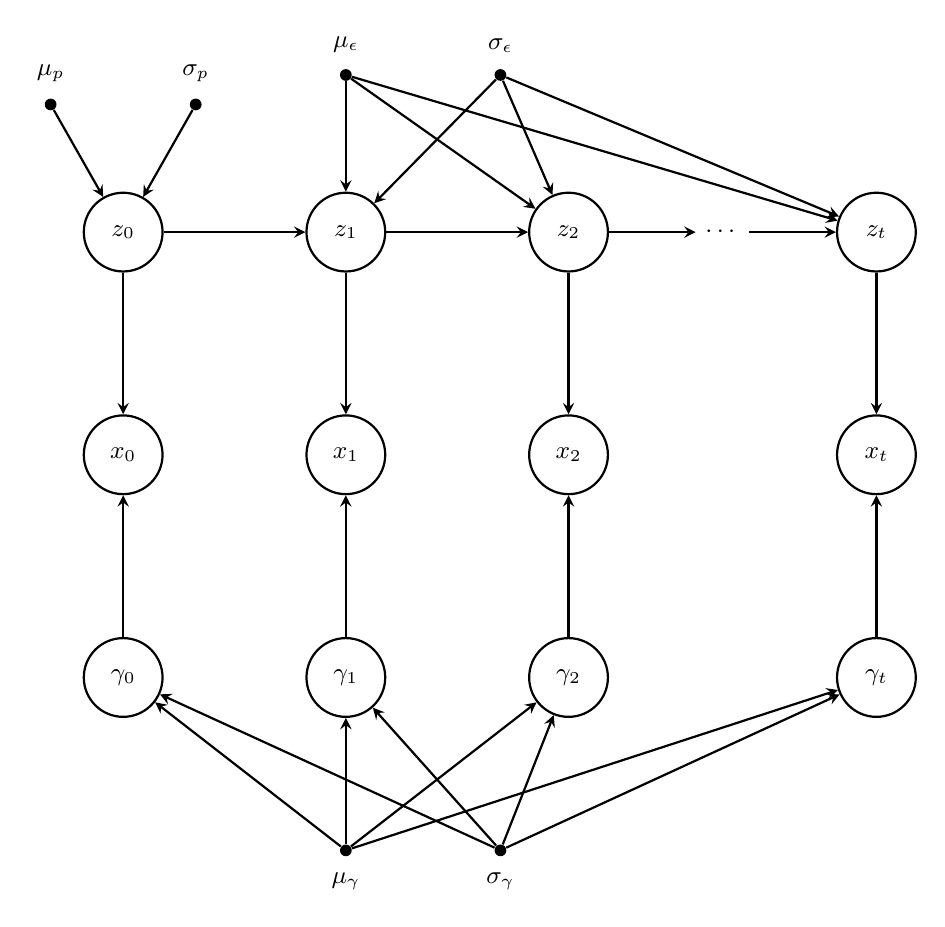
\begin{tikzpicture}[
        >=stealth,
        node distance=1.8cm and 1.8cm,
        latent/.style={circle, draw, thick, minimum size=1cm, inner sep=0pt},
        obs/.style={circle, draw, thick, minimum size=1cm, inner sep=0pt},
        noise/.style={circle, fill=black, inner sep=1.5pt},
        every node/.style={font=\small}
    ]
    
    % Hidden states
    \node[latent] (z0) {$z_0$};
    \node[latent, right=of z0] (z1) {$z_1$};
    \node[latent, right=of z1] (z2) {$z_2$};
    \node[right=1.1cm of z2] (dots1) {$\cdots$};
    \node[latent, right=1.1cm of dots1] (zt) {$z_t$};
    
    % Observations
    \node[obs, below=of z0] (x0) {$x_0$};
    \node[obs, below=of z1] (x1) {$x_1$};
    \node[obs, below=of z2] (x2) {$x_2$};
    \node[obs, below=of zt] (xt) {$x_t$};
    
    % Emission noises
    \node[latent, below=of x0] (g0) {$\gamma_0$};
    \node[latent, below=of x1] (g1) {$\gamma_1$};
    \node[latent, below=of x2] (g2) {$\gamma_2$};
    \node[latent, below=of xt] (gt) {$\gamma_t$};
    
    % Prior parameters
    \node[noise, above left=1.2cm and 0.5cm of z0] (muzp) {};
    \node[noise, above right=1.2cm and 0.5cm of z0] (sigzp) {};
    \node[above=0.08cm of muzp] {$\mu_{p}$};
    \node[above=0.08cm of sigzp] {$\sigma_{p}$};
    
    % Transition noise parameters
    \node[noise, above=1.4cm of z1] (mueps) {};
    \node[noise, right=1.8cm of mueps] (sigeps) {};
    \node[above=0.08cm of mueps] {$\mu_\epsilon$};
    \node[above=0.08cm of sigeps] {$\sigma_\epsilon$};
    
    % Emission noise parameters
    \node[noise, below=1.6cm of g1] (mugam) {};
    \node[noise, right=1.8cm of mugam] (siggam) {};
    \node[below=0.08cm of mugam] {$\mu_\gamma$};
    \node[below=0.08cm of siggam] {$\sigma_\gamma$};
    
    % State chain
    \draw[->, thick] (z0) -- (z1);
    \draw[->, thick] (z1) -- (z2);
    \draw[->, thick] (z2) -- (dots1);
    \draw[->, thick] (dots1) -- (zt);
    
    % Emissions
    \draw[->, thick] (z0) -- (x0);
    \draw[->, thick] (z1) -- (x1);
    \draw[->, thick] (z2) -- (x2);
    \draw[->, thick] (zt) -- (xt);
    
    % Noise into observations
    \draw[->, thick] (g0) -- (x0);
    \draw[->, thick] (g1) -- (x1);
    \draw[->, thick] (g2) -- (x2);
    \draw[->, thick] (gt) -- (xt);
    
    % Prior parameters into z0
    \draw[->, thick] (muzp) -- (z0);
    \draw[->, thick] (sigzp) -- (z0);
    
    % Transition noise parameters into all z_1,...,z_t
    \foreach \target in {z1,z2,zt} {
        \draw[->, thick] (mueps) -- (\target);
        \draw[->, thick] (sigeps) -- (\target);
    }
    
    % Emission noise parameters into all gamma_t
    \foreach \target in {g0,g1,g2,gt} {
        \draw[->, thick] (mugam) -- (\target);
        \draw[->, thick] (siggam) -- (\target);
    }
    
    \end{tikzpicture}
\end{center}
 

\begin{enumerate}
  \item In this first part, we will walk through the derivation of the conditional distribution of $z_t|(x_0, \cdots, x_{t})$.
  \begin{enumerate}
      \item How does the quantity $p(z_t| x_0, \cdots, x_{t})$ relate to $\alpha_t(z_t)$ and $\beta_t(z_t)$ from the forward-backward algorithm for HMMs?  What is the operation we are performing called?
      \item The above quantity $p(z_t|x_0, \cdots, x_t)$ is the PDF for a Normal distribution with mean $\mu_t$ and variance $\sigma_t^2$. We start our derivation of $\mu_t$ and $\sigma_t^2$ by writing:
      \begin{align*}
          p(z_t|x_0, \cdots, x_t) \propto p(x_t|z_t)p(z_t|x_0, \cdots x_{t-1})
      \end{align*}
      What is $p(x_t|z_t)$ equal to?
      \item Suppose we are given the mean and variance of the distribution $z_{t-1}|(x_0, \cdots, x_{t-1})$ as $\mu_{t-1}$, $\sigma^2_{t-1}$. What is $p(z_t|x_0, \cdots x_{t-1})$ equal to? 
      
      \textbf{Hint 1}: Start by marginalizing out over $z_{t-1}$.
      
      \textbf{Hint 2}: You may cite the fact that 
      \[\int N(y-x ; \mu_a, \sigma^2_a)N(x ; \mu_b, \sigma^2_b)dx = N(y ; (\mu_a + \mu_b), (\sigma^2_a + \sigma^2_b))\]
      \item Combine your answers from parts (b) and (c) to get a final expression for $p(z_t|x_0, \cdots, x_t)$. Report the mean $\mu_t$ and variance $\sigma_t^2$ of this Normal.

      \textbf{Hint 1}: Rewrite $N(x_t; z_t, \siggam^2)$ as $N(z_t; x_t, \siggam^2)$.
      
      \textbf{Hint 2}: You may cite the fact that 
      \[N(x; \mu_a, \sigma^2_a)N(x; \mu_b, \sigma^2_b) \propto N\left(x; \frac{\sigma^2_b}{\sigma^2_a+\sigma^2_b}\mu_a + \frac{\sigma^2_a}{\sigma^2_a+\sigma^2_b}\mu_b, \ \left(\frac{1}{\sigma^2_a} + \frac{1}{\sigma^2_b}\right)^{-1}\right)\]
  \end{enumerate}
  \item In a sentence or two, interpret $\mu_t$ in terms of how it combines observations from the past with the current observation. 
\end{enumerate}
\end{problem}


\newpage

\begin{solution}
	Your solution here.
\end{solution}

\newpage







\begin{problem}[Policy and Value Iteration, 15 pts]

You have a robot that you wish to collect two parts in an environment and bring them to a goal location. There are also parts of the environment that you wish the robot avoid to reduce wear on the floor. \\

\noindent \textbf{Environment model.} Eventually, you settle on the following way to model the environment as a Gridworld.  The ``states'' in Gridworld are represented by locations in a two-dimensional space.  Here we show each state and its reward:

\begin{center}
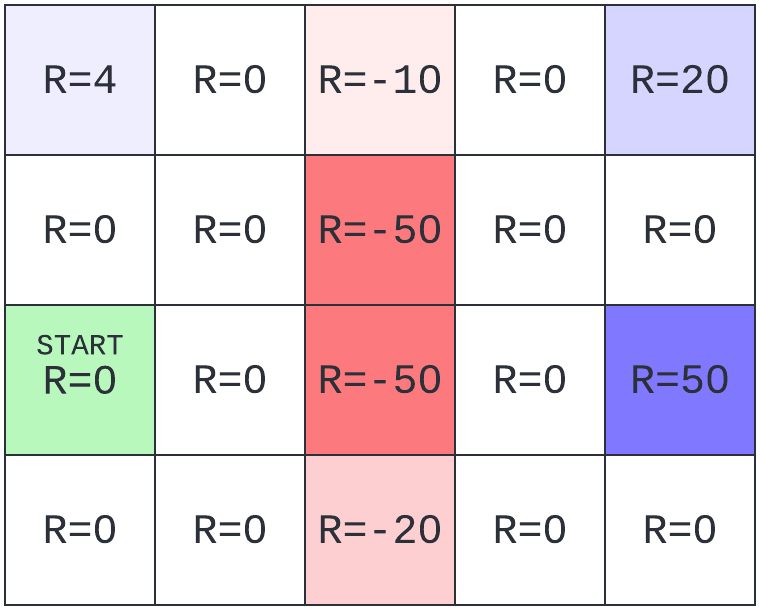
\includegraphics[width=3in]{img_input/gridworld.png}
\end{center}

The set of actions is \{N, S, E, W\}, which corresponds to moving north (up), south (down), east (right), and west (left) on the grid. Taking an action in Gridworld does not always succeed with probability $1$; instead the agent has probability $0.1$ of ``slipping'' into a state on either side, but not backwards. For example, if the agent tries to move right from START, it succeeds with probability 0.8, but the agent may end up moving up or down with probability 0.1 each. Also, the agent cannot move off the edge of the grid, so moving left from START will keep the agent in the same state with probability 0.8, but also may slip up or down with probability 0.1 each. Lastly, the agent has no chance of slipping off the grid, so moving up from START results in a 0.9 chance of success with a 0.1 chance of moving right.

Also, the agent does not receive the reward of a state immediately upon entry, but instead only after it takes an action at that state. For example, if the agent moves right four times (deterministically, with no chance of slipping) the rewards would be +0, +0, -50, +0, and the agent would reside in the +50 state. Regardless of what action the agent takes here, the next reward would be +50. \\

\noindent \textbf{Action items.} In this problem, you will first implement policy and value iteration in this setting and discuss the policies that you find.  Next, you will interrogate whether this approach to modeling the original problem was appropriate.

Your job is to implement the following three methods in file \texttt{homework6.ipynb}. Please use the provided helper functions \texttt{get\_reward} and \texttt{get\_transition\_prob} to implement your solution. \emph{Do not use any outside code.} \\

\noindent \textbf{Important note.} The state space is represented using integers, which range from 0 (the top left) to 19 (the bottom right). Therefore both the policy \texttt{pi} and the value function \texttt{V} are 1-dimensional arrays of length \texttt{num\_states = 20}. Your policy and value iteration methods should only implement one update step of the iteration - they will be repeatedly called by the provided \texttt{learn\_strategy} method to learn and display the optimal policy. You can change the number of iterations that your code is run and displayed by changing the $\texttt{max\_iter}$ and $\texttt{print\_every}$ parameters of the $\texttt{learn\_strategy}$ function calls at the end of the code.

Note that we are doing infinite-horizon planning to maximize the expected reward of the traveling agent. For parts 1-3, set discount factor $\gamma = 0.7$.

\begin{enumerate}
    \item First, on policy iteration. Note that you do not need submit anything in your write-up for 1(a) and 1(b).
    \begin{enumerate}
        \item Implement function \texttt{policy\_evaluation}.  Your solution should learn value function $V$, either using a closed-form expression or iteratively using convergence tolerance $\texttt{theta = 0.0001}$ (i.e., if $V^{(t)}$ represents $V$ on the $t$-th iteration of your policy evaluation procedure, then if $|V^{(t + 1)}[s] - V^{(t)}[s]| \leq \theta$ for all $s$, then terminate and return $V^{(t + 1)}$.)
    
        \item Implement function \texttt{update\_policy\_iteration} to update the policy \texttt{pi} given a value function \texttt{V} using \textbf{one step} of policy iteration.
        
        \item Set \texttt{max\_iter = 4}, \texttt{print\_every = 1} to show the learned value function and the associated policy for the first 4 policy iterations. Do not modify the plotting code. Please fit all 4 plots onto one page of your writeup.
        
        \item Set \texttt{ct = 0.01} and increase \texttt{max\_iter} such that the algorithm converges. Include a plot of the final learned value function and policy. How many iterations does it take to converge? Now if we try \texttt{ct = 0.001} and \texttt{ct = 0.0001}, how does this affect the number of iterations until convergence?
    \end{enumerate}
      
    \item Next, on value iteration.
    \begin{enumerate}
        \item Implement function \texttt{update\_value\_iteration}, which performs \textbf{one step} of value iteration to update \texttt{V}, \texttt{pi}.
          
        \item Set \texttt{max\_iter = 4}, \texttt{print\_every = 1} to show the learned value function and the associated policy for the first 4 value iterations. Do not modify the plotting code. Please fit all 4 plots onto one page of your writeup.
        
        \item Set \texttt{ct = 0.01} and increase \texttt{max\_iter} such that the algorithm converges. Include a plot of the final learned value function and policy. How many iterations does it take to converge? Now try \texttt{ct = 0.001} and \texttt{ct = 0.0001}. How does this affect the number of iterations until convergence?
    \end{enumerate}
    
    \item Plot the learned policy with each of $\gamma \in (0.6,0.7,0.8,0.9)$. Include all 4 plots in your writeup. Describe in one paragraph how the observed policies differ and possible explanations.
    
    \item Now suppose that the game ends at any state with a positive reward, i.e. it immediately transitions you to a new state with zero reward that you cannot transition away from. What do you expect the optimal policy to look like, as a function of gamma? Numerical answers are not required, intuition is sufficient.
 
    \item In this problem, we came up with a model for the problem, solved it, and then we had a policy to use on the real robot. What is the value of the approach we took, compared to, e.g., using RL on the robot to identify a policy that achieved your objective? What are some limitations of our modeling approach (which may also apply to RL)?
\end{enumerate}
\end{problem}

\newpage

\begin{solution}
	Your solution here.
\end{solution}



\newpage





\begin{problem}[Reinforcement Learning, 20 pts]
    In 2013, the mobile game \emph{Flappy Bird} took the world by storm. You'll be developing a Q-learning agent to play a similar game, \emph{Swingy Monkey} (See Figure~\ref{fig:swingy}).  In this game, you control a monkey that is trying to swing on vines and avoid tree trunks.  You can either make him jump to a new vine, or have him swing down on the vine he's currently holding.  You get points for successfully passing tree trunks without hitting them, falling off the bottom of the screen, or jumping off the top.  There are some sources of randomness: the monkey's jumps are sometimes higher than others, the gaps in the trees vary vertically, the gravity varies from game to game, and the distances between the trees are different.  You can play the game directly by pushing a key on the keyboard to make the monkey jump.  However, your objective is to build an agent that \emph{learns} to play on its own. % As a note, you will need to install the \verb|pygame| module (\url{http://www.pygame.org/wiki/GettingStarted}). 
    \\
  
    \noindent \textbf{Task:} Your task is to use Q-learning to find a policy for the monkey that can navigate the trees.  The \verb|homework6_soln.ipynb| file contains starter code for setting up your learner that interacts with the game. This is the \textbf{only code file} you need to modify. At the beginning of the code, you will import the \verb|SwingyMonkey| class, which is the implementation of the game that has already been completed for you. Note that by default we have you import this class from the file \verb|SwingyMonkeyNoAnimation.py|, which allows you to speed up testing. To actually see the game animation, you can instead import from \verb|SwingyMonkey.py|. Additionally, we provide a video of the staff Q-Learner playing the game at \url{https://youtu.be/xRD6xBQbauw}. It figures out a reasonable policy in a few iterations. 
    
    You'll be responsible for implementing the Python function  \verb|action_callback|. The action callback will take in a dictionary that describes the current state of the game and return an action for the next time step. This will be a binary action, where 0 means to swing downward and 1 means to jump up. The dictionary you get for the state looks like this:
    \begin{csv}
    { 'score': <current score>,
      'tree': { 'dist': <pixels to next tree trunk>,
                'top':  <height of top of tree trunk gap>,
                'bot':  <height of bottom of tree trunk gap> },
      'monkey': { 'vel': <current monkey y-axis speed>,
                  'top': <height of top of monkey>,
                  'bot': <height of bottom of monkey> }}
    \end{csv}
    All of the units here (except score) will be in screen pixels. Figure~\ref{fig:swingy-ann} shows these graphically. Note that since the state space is very large (effectively continuous), the monkey's relative position needs to be discretized into bins. The pre-defined function \verb|discretize_state| does this for you. \\

    \noindent \textbf{Requirements}
    \\
    \noindent \textit{Code}: First, you should implement Q-learning with an
    $\epsilon$-greedy policy yourself. You can increase the performance by
    trying out different parameters for the learning rate $\alpha$,
    discount rate $\gamma$, and exploration rate $\epsilon$. \emph{Do not use outside RL code for this assignment.} Second, you should use a method of your choice to further improve the performance. This could be inferring gravity at each epoch (the gravity varies from game to game), updating the reward function, trying decaying epsilon greedy functions (this method in particular is highly recommended), changing the features in the state space, and more. The minimum expectation to have an agent that reaches scores over 50 at least once before the 100th epoch. \\
    
    \noindent \textit{Evaluation}: In 1-2 paragraphs, explain how your agent performed and what decisions you made and why. Make sure to provide evidence where necessary to explain your decisions. You must include in your write up at least one plot or table that details the performances of parameters tried (i.e. plots of score vs. epoch number for different parameters). \\
    
    \noindent \textit{Note}: Note that you can simply discretize the state and action spaces and run the Q-learning algorithm. There is no need to use complex models such as neural networks to solve this problem.
    \begin{figure}[H]
        \centering
        \subfloat[SwingyMonkey Screenshot]{%
            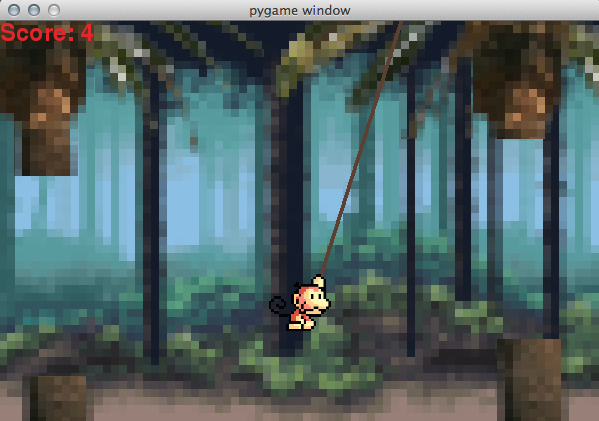
\includegraphics[width=0.45\linewidth]{img_input/swingy}
            \label{fig:swingy}
        }\hfill
        \subfloat[SwingyMonkey State]{%
            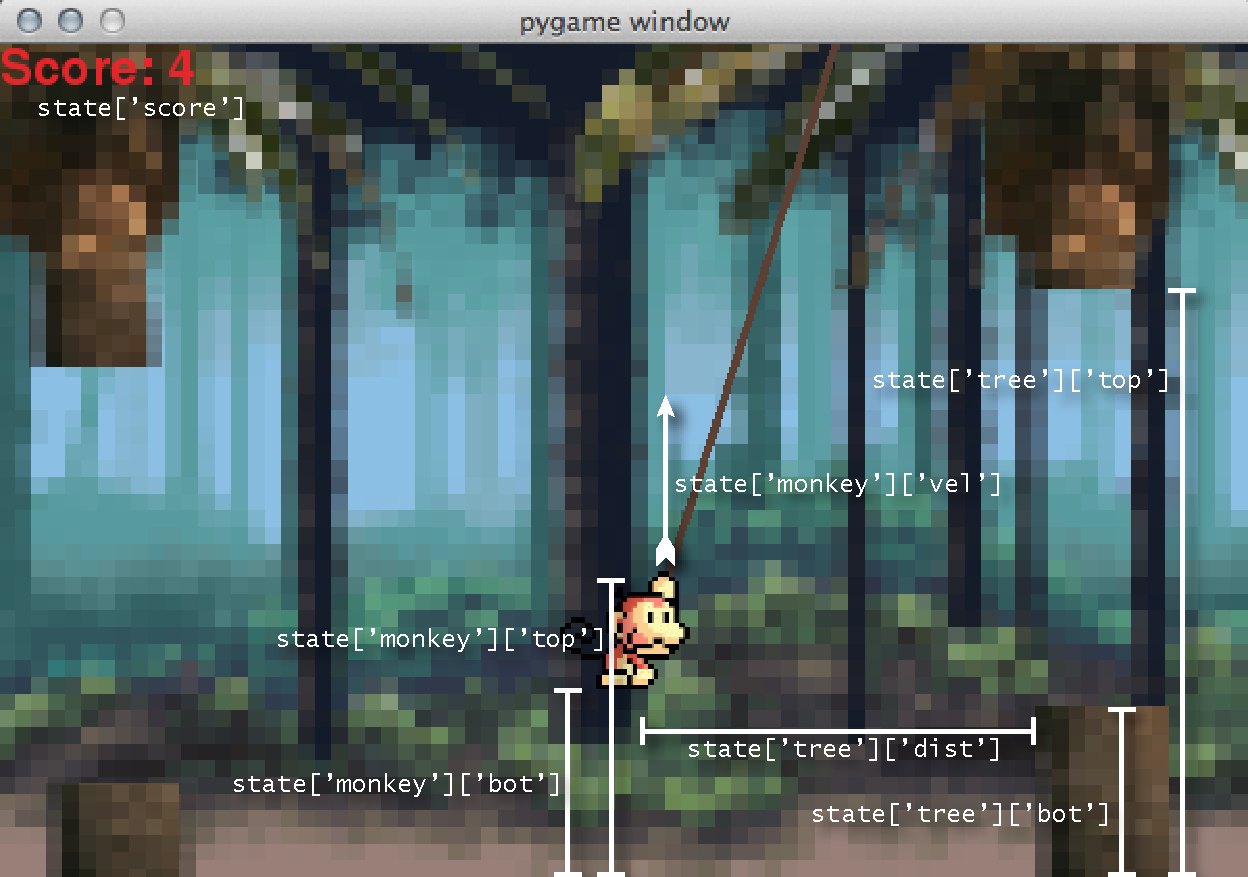
\includegraphics[width=0.45\linewidth]{img_input/swingy-ann}
            \label{fig:swingy-ann}
        }
        \caption{(a) Screenshot of the Swingy Monkey game.  (b) Interpretations of various pieces of the state dictionary.}
    \end{figure}
\end{problem}
    

\begin{solution}
	Your solution here.
\end{solution}

\newpage

\newpage

\begin{problem}[Autoregressive Models, 20 pts]
An autoregressive model factorizes a joint distribution over a sequence $\mathbf{x} = (x_1, \ldots, x_T)$ using the chain rule of probability:
\[
p(x_1, \ldots, x_T) \;=\; \prod_{t=1}^{T} p(x_t \mid x_{<t}).
\]
In this problem you will examine three consequences of the sequential structure of autoregressive generation. Part 1 concerns the algorithmic cost of finding the most probable sequence. Part 2 concerns the computational cost of each generation step and how the causal structure of a Transformer permits caching. Part 3 introduces speculative decoding, a technique used in modern LLM inference to partially parallelize generation.
\end{problem}

\begin{framed}
\noindent \textbf{Part 1: Decoding autoregressive models.}

\noindent Consider the following autoregressive model over sequences $\mathbf{x} = (x_1, x_2, x_3)$ with each $x_t \in \{A, B\}$:
\begin{align*}
  p(x_1 = A) &= 0.6, \qquad p(x_1 = B) = 0.4 \\
  p(x_2 = A \mid x_1 = A) &= 0.7, \qquad p(x_2 = B \mid x_1 = A) = 0.3 \\
  p(x_2 = A \mid x_1 = B) &= 0.1, \qquad p(x_2 = B \mid x_1 = B) = 0.9 \\
  p(x_3 = A \mid A, A) &= 0.6, \qquad p(x_3 = B \mid A, A) = 0.4 \\
  p(x_3 = A \mid A, B) &= 0.5, \qquad p(x_3 = B \mid A, B) = 0.5 \\
  p(x_3 = A \mid B, A) &= 0.5, \qquad p(x_3 = B \mid B, A) = 0.5 \\
  p(x_3 = A \mid B, B) &= 0.05, \qquad p(x_3 = B \mid B, B) = 0.95
\end{align*}

\begin{enumerate}
  \item[1a.] \emph{Greedy decoding} selects $x_t = \arg\max_{x} p(x \mid x_{<t})$ at each step. Compute the sequence $\mathbf{x}^{\text{greedy}}$ produced by greedy decoding, and report its joint probability.
  
  \item[1b.] \emph{Maximum a posteriori (MAP) decoding} returns $\mathbf{x}^{\star} = \arg\max_{\mathbf{x}} p(\mathbf{x})$. Enumerate all 8 sequences and report $\mathbf{x}^{\star}$ and its probability.
  
  \item[1c.] The Viterbi algorithm finds the most-probable hidden-state sequence for a Hidden Markov Model in $\mathcal{O}(TK^2)$ time, where $K$ is the number of hidden states. Exact MAP decoding for a general autoregressive model of length $T$ with vocabulary size $V$ requires $\mathcal{O}(V^T)$ time.

  Now consider a restricted autoregressive model in which each token depends only on the previous $k$ tokens: $p(x_t \mid x_{<t}) = p(x_t \mid x_{t-k}, \ldots, x_{t-1})$ for all $t > k$. For this restricted model, exact MAP decoding can be done in polynomial time using dynamic programming. You will design the algorithm.

  Let $\delta_t(\mathbf{w})$ denote the probability of the most-probable sequence of length $t$ that ends in the window $\mathbf{w} = (x_{t-k+1}, \ldots, x_t)$.
  
  \begin{enumerate}
    \item[(i)] How many possible values of $\mathbf{w}$ are there?
    \item[(ii)] Write the recursion that expresses $\delta_{t+1}$ in terms of $\delta_t$.
    \item[(iii)] Using your recursion, state the total time to compute all $\delta_T$ values, as a function of $T$, $V$, and $k$. Verify that $k = 1$ recovers the $\mathcal{O}(TV^2)$ Viterbi bound, and that $k = T-1$ recovers brute-force enumeration.
  \end{enumerate}
\end{enumerate}
\end{framed}

\newpage

\begin{framed}
\noindent \textbf{Part 2: KV caching.}

\noindent A Transformer language model processes a sequence by computing, for each position $t$, a representation $h_t$ of the token at that position. From each $h_t$ it derives a key $K_t = W_K h_t$ and a value $V_t = W_V h_t$, using learned projection matrices $W_K$ and $W_V$. Causal self-attention then combines the keys and values from all positions $1, \ldots, t$ to produce the model's output at position $t$.

In autoregressive generation, the model starts from a prefix $x_1, \ldots, x_T$ and generates new tokens one at a time. To generate $x_{T+1}$, the model runs a forward pass and samples from the output distribution at position $T$. Then $x_{T+1}$ is appended to the sequence, and the model runs again to generate $x_{T+2}$. And so on, until $k$ new tokens have been generated.

In a naive implementation, each of the $k$ generation steps recomputes every $K_t$ and $V_t$ from scratch. But notice: the value of $K_t$ for a position $t$ already in the sequence does not change when a later token is appended. So we can compute each $K_t$ and $V_t$ just once and cache them, looking up the cached values on subsequent steps rather than recomputing. This optimization is called \emph{KV caching} and is standard in every production language model inference system. You will analyze its computational benefit.

\begin{enumerate}
  \item[2a.] Consider the naive generation procedure, in which each of the $k$ generation steps runs a full Transformer forward pass over the entire current sequence (no caching).
  
  Let $N_{\text{naive}}(T, k)$ denote the total number of key computations $W_K h_t$ performed across all $k$ generation steps.
  
  \begin{enumerate}
    \item[(i)] Just before generating $x_{T+j}$, how long is the sequence the model is processing, and how many key computations does that forward pass require?
    \item[(ii)] Sum your answer over $j = 1, \ldots, k$ to get a closed-form expression for $N_{\text{naive}}(T, k)$. Show that $N_{\text{naive}}(T, k) = \mathcal{O}((T+k)^2)$.
  \end{enumerate}
  
  \item[2b.] KV caching relies on a specific property of causal self-attention. What is the property, and why does it hold? Why does the same caching break down under bidirectional self-attention?
  
  \item[2c.] Now consider generation with KV caching. Before the first generation step, the model performs a single forward pass over the initial prefix $x_1, \ldots, x_T$ to compute and store $K_t$ and $V_t$ for each position $t = 1, \ldots, T$. This is called the \emph{prefill} phase. Thereafter, at each of the $k$ generation steps, the model computes only the key and value for the single newly appended token, and reuses the cached keys and values for all earlier positions.
  
  Let $N_{\text{cached}}(T, k)$ denote the total number of key computations $W_K h_t$ performed across the prefill and all $k$ generation steps.
  
  \begin{enumerate}
    \item[(i)] Give a closed-form expression for $N_{\text{cached}}(T, k)$.
    \item[(ii)] State the ratio $N_{\text{naive}}(T, k) / N_{\text{cached}}(T, k)$ in the regime $k \gg T$ (long generations from short prompts).
  \end{enumerate}
  
  \item[2d.] A single training forward pass over a sequence of length $k$ takes roughly the same wall-clock time as generating just one new token during inference - even though the training pass does far more total arithmetic.
  
  Why does training parallelize across positions while generation does not? Does KV caching help during training?
\end{enumerate}
\end{framed}

\newpage

\begin{framed}
\noindent \textbf{Part 3: Speculative decoding.}

\noindent Part 2 showed that generation is slow because it cannot be parallelized: each token must be sampled before the next can be computed. \emph{Speculative decoding} is a technique that partially sidesteps this constraint by using two models: a large \emph{target} model $p$ whose distribution we want to sample from, and a small \emph{draft} model $q$ that approximates $p$ but is much cheaper to run.

Each round of speculative decoding proceeds as follows:

\begin{enumerate}
  \item[(i)] \textbf{Drafting.} The draft model $q$ generates $k$ candidate tokens $x_{T+1}, \ldots, x_{T+k}$ autoregressively. This is cheap because $q$ is small.
  \item[(ii)] \textbf{Verification.} The target model $p$ runs a single forward pass over the sequence $(x_1, \ldots, x_{T+k})$, producing the target distributions $p(\cdot \mid x_1, \ldots, x_{T+i-1})$ for every $i$ from 1 to $k+1$ in parallel. The first $k$ of these distributions are used to verify the drafts; the last one is a ``bonus'' distribution at position $T+k+1$, used in step (iii) if all drafts are accepted.
  \item[(iii)] \textbf{Acceptance.} The draft tokens are considered one at a time. Draft token $x_{T+i}$ is accepted with probability
  \[
  \min\!\left(1, \ \frac{p(x_{T+i} \mid x_1, \ldots, x_{T+i-1})}{q(x_{T+i} \mid x_1, \ldots, x_{T+i-1})}\right).
  \]
  If $x_{T+i}$ is rejected, all subsequent drafts $x_{T+i+1}, \ldots, x_{T+k}$ are discarded, and a replacement token is sampled at position $T+i$ from a distribution constructed so that the output sequence still matches $p$.
\end{enumerate}

Under this acceptance rule, the sequence of tokens output by speculative decoding has the same distribution as if we had generated from the target $p$ directly. Speculative decoding preserves the target distribution exactly.

\begin{enumerate}
  \item[3a.] In the verification step, the target model produces $k$ conditional distributions in a single forward pass, while generating those same $k$ tokens from the target model alone would require $k$ sequential forward passes.
  
  \begin{enumerate}
    \item[(i)] What property of the target model's forward pass makes parallel verification possible? Why does the same property not enable parallel generation?
    \item[(ii)] Suppose the draft model and the target model are identical, so $q = p$. What happens to speculative decoding? Is there any speedup, or any additional cost? Explain.
  \end{enumerate}
  
  \item[3b.] The acceptance probability for draft token $x_{T+i}$ is
  \[
  \min\!\left(1, \ \frac{p(x_{T+i} \mid x_1, \ldots, x_{T+i-1})}{q(x_{T+i} \mid x_1, \ldots, x_{T+i-1})}\right).
  \]
  
  \begin{enumerate}
    \item[(i)] When $p(x_{T+i} \mid x_1, \ldots, x_{T+i-1}) \geq q(x_{T+i} \mid x_1, \ldots, x_{T+i-1})$, what is the acceptance probability? Why does it make sense to always accept in this case?
    \item[(ii)] When $p(x_{T+i} \mid x_1, \ldots, x_{T+i-1}) \ll q(x_{T+i} \mid x_1, \ldots, x_{T+i-1})$, what is the acceptance probability? Why does it make sense to usually reject?
  \end{enumerate}
\end{enumerate}
\end{framed}

\newpage

\begin{solution}
	Your solution here.
\end{solution}

\newpage

\begin{problem}[Embedded Ethics, 10 pts]
    One aim of the class session on Fairness in Model Selection was to show that we often need to consider the broader socio-technical context when using our CS expertise to solve real-world problems. This is just as true in the case of reinforcement learning. To practice this skill of considering the broader socio-technical context, answer the following prompt in a few sentences (at most 250 words). Answers should exhibit some careful thought about the socio-technical context, but don't need to be comprehensive. \\

    \noindent Social media platforms like Facebook, TikTok, and X make extensive use of reinforcement learning, and many scholars have argued that widespread engagement with these platforms has contributed to political polarization, where users with a particular political leaning develop more extreme views over time. Assume users of a particular platform do in fact tend to develop more extreme political views over time. Using what you've learned about RL, devise a possible explanation for how the particular reward function the app's creators chose may have contributed to this problematic increase in political polarization.
\end{problem}

\begin{solution}
	Your solution here.
\end{solution}

\newpage
%%%%%%%%%%%%%%%%%%%%%%%%%%%%%%%%%%%%%%%%%%%%%
% Name and Calibration
%%%%%%%%%%%%%%%%%%%%%%%%%%%%%%%%%%%%%%%%%%%%%
\newpage
\subsection*{Name}
\subsection*{Collaborators and Resources}
Whom did you work with, and did you use any resources beyond cs181-textbook and your notes?

\end{document}
